\section{Results and Discussion}\label{sec:Results}

\subsection{The Square Well Potential}
The phase shift of the square well is found by VPA and compared to the analytical form.
A well with the arbitrary depth of \(V_{0}=4.0\) is used as
example, with the computed curves shown in~\cref{fig:analyticalcot}. The curves
overlap, but the analytical solution
has a jump at \(k\approx 2.8\), stemming from the inherent modulo \(\pi\)
ambiguity. The transformation \(k\cot\delta\) lifts this ambiguity while fixing
the phase shift to \(0\) at \(k=0\), plotted in the lower panel of the figure.
Once transformed the curves overlap perfectly, as expected.

\begin{figure}[ht!]
  \showthe\columnwidth % Use this to determine the width of the figure.
  \showthe\textwidth % Use this to determine the width of the figure.
  \centering
  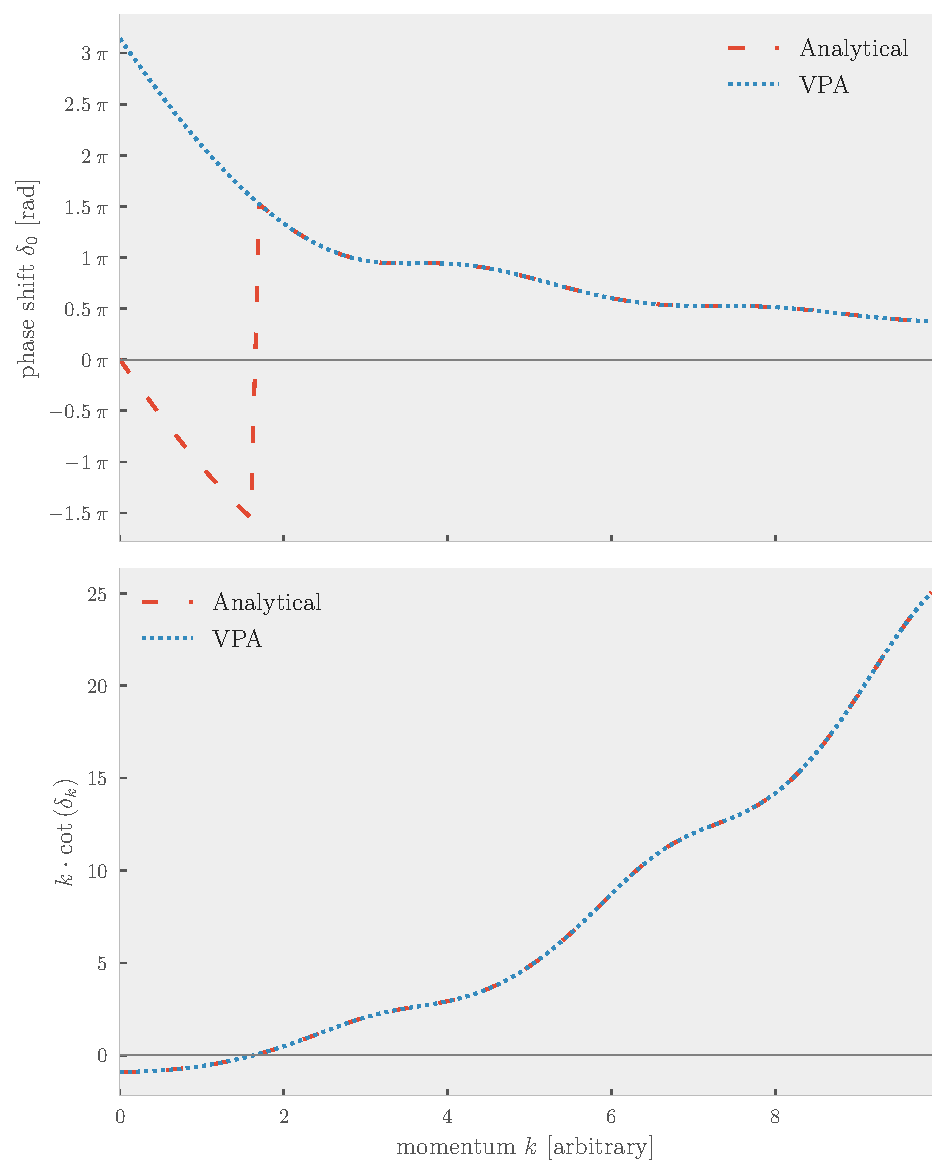
\includegraphics[]{Figures/analytical_cot.pdf}
  \caption{\label{fig:analyticalcot}The \(s\)-wave phase shift for a square well
    potential \(V=-4\) MeV, and reduced mass of \(1\) MeV. The \(\pi\)-ambiguity
  in the analytical solution is lifted in the lower panel with the
  transformation \(k\cot{\delta_{0}}\), showing a perfect overlap.}
\end{figure}

The simple form the square well potential allows us to illustrate some general
behaviors of the phase shift. The phase shifts produced by several
different well depths are plotted
in~\cref{fig:squarewellwave} together with the corresponding cross sections 
in the lower panel. As \(k\to 0\), all curves approach an integral multiple of
\(\pi\), and decrease towards zero as \(k\to \infty\). As
Levinson's theorem dictates, the multiple of \(\pi\) corresponds to the number
of bound states each well can contain, with
the number of states increasing as the potential deepens.

For some particular well depths, the cross-sections shoot up beyond the limits of
the plot. The phase shift curves too have a
characteristic shape, rising rapidly as they approach \(k=0\). Examples are marked by dashed
lines. From our expos\'e on resonances in~\cref{sec:resonances}, we recognize these
as zero energy resonances. Such curves indicate that the
potential is on the verge of allowing for an additional bound state, producing a
metastable state with cross-sections approaching the unitarity bound. Indeed, increasing the depth slightly makes the phase shift jump up
to the next integral value.

A related phenomenon happens where the phase shift crosses \(\delta=\pi\), at
which point the cross-section falls off to zero. This is more
clearly demonstrated in~\cref{fig:pizero}. A phase shift of \(n\pi\) means the wave inside
the well has precisely \(n\) more oscillations than the free wave. When the scattered
wave exits the potential, it is exactly in phase with the free wave, and hence
indistinguishable. If the higher \(l>0\) waves are negligible in the same region,
the potential causes no scattering at all. This is the cause for the
\textit{Ramsauer-Townsend effect}\cite[p.~195]{taylor}, where certain gases are completely
transparent for electrons at a given energy.
% \begin{figure}[ht]
%   \centering
%   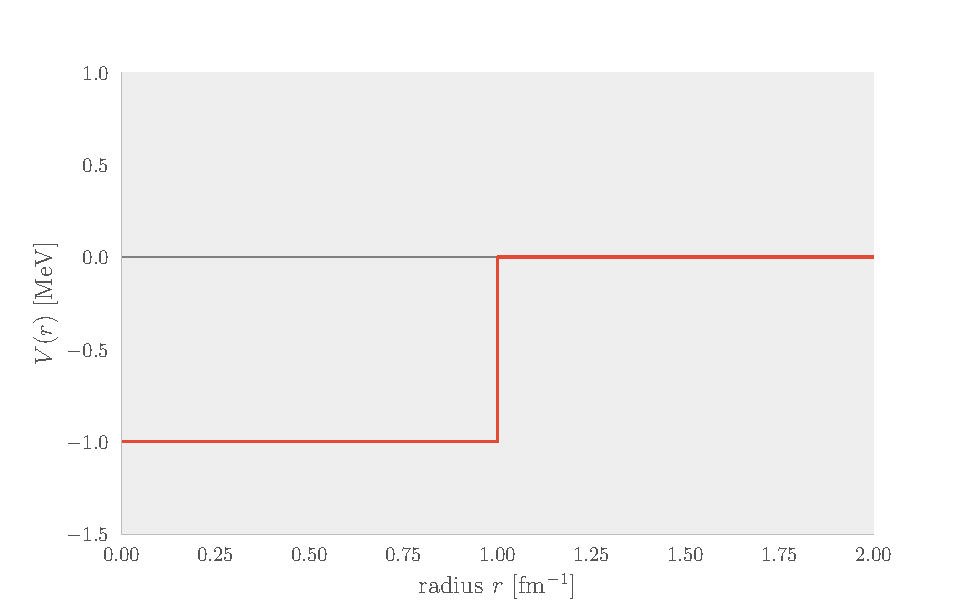
\includegraphics[]{Figures/squarewell.pdf}
%   \caption{\label{fig:squarewell} }
% \end{figure}

\begin{figure}[hp]
  \centering
  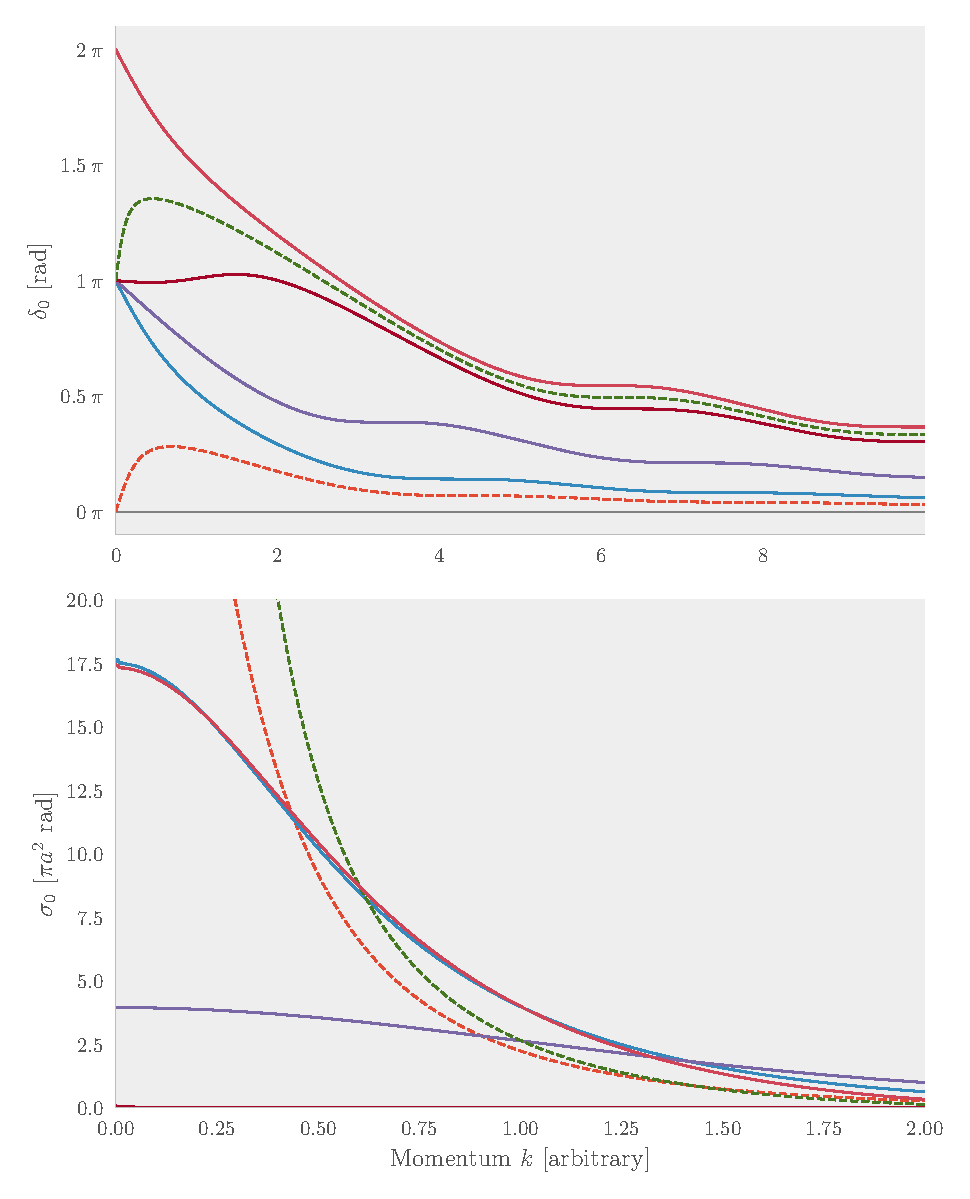
\includegraphics[]{Figures/square_well_wave.pdf}
  \caption{\label{fig:squarewellwave}The phase shift and corresponding cross
    section for several square wells of different depths. All curves fall off to
    zero by definition. As the wells deepen,
    the number of possible bound states increases, manifesting as curves
    starting at larger multiples of \(\pi\). The dashed lines show the zero energy peaks.}
\end{figure}

\begin{figure}[hp]
  \centering
  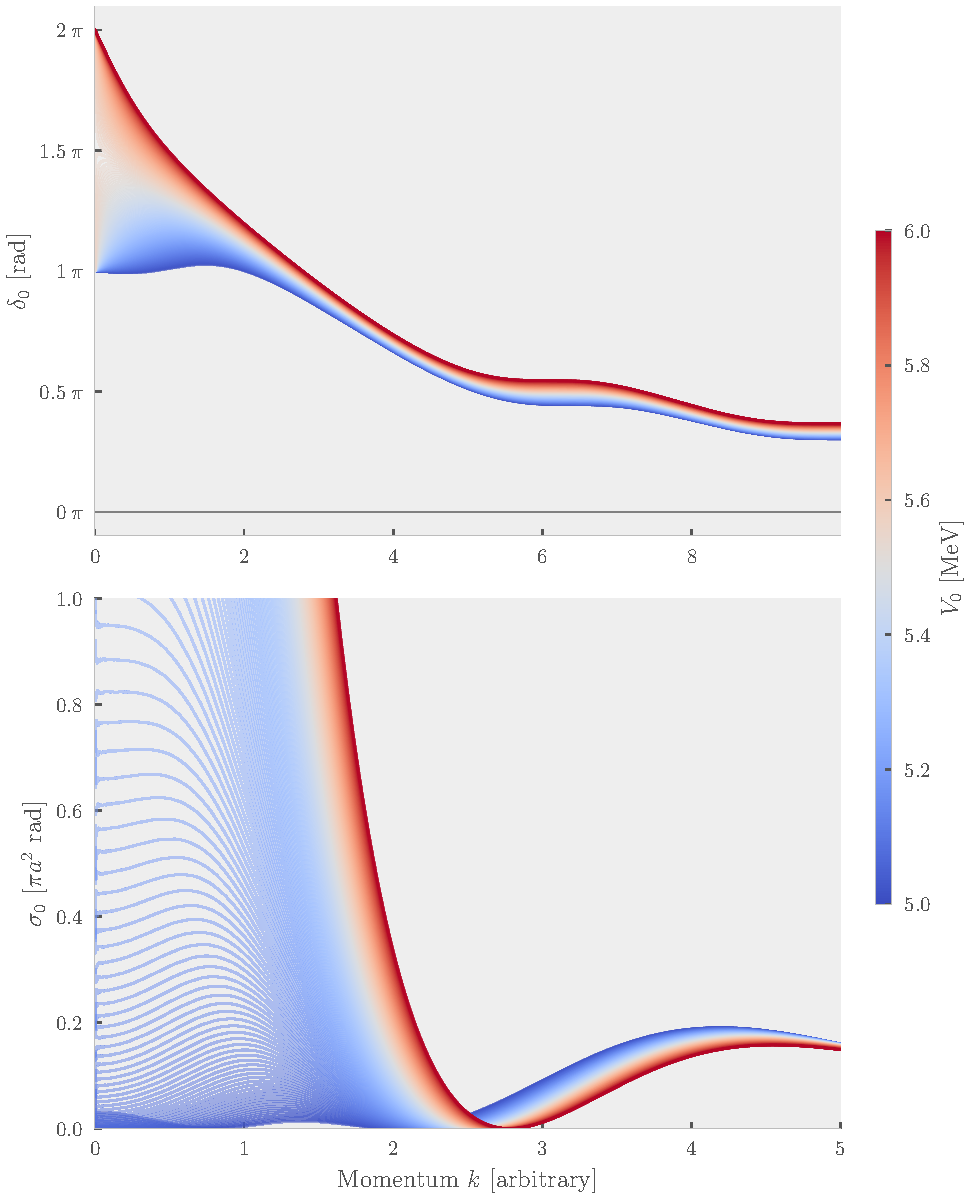
\includegraphics[]{Figures/square_well_wave_pi.pdf}
  \caption{\label{fig:pizero}Examples of phase shift curves crossing \(\delta =
    \pi\). The scattered wave gets in phase with the free wave, ending up being equivalent
    with no scattering. The cross section plummets to zero when this happens.}
\end{figure}

For check that the method handles repulsive potentials, the phase shift is found for positive wells, see~\cref{fig:positivesquare}. We expect there to be no bound states, and for
the phase shift to be negative. This is indeed the case, as the figure shows.

\begin{figure}[ht!]
  \centering
  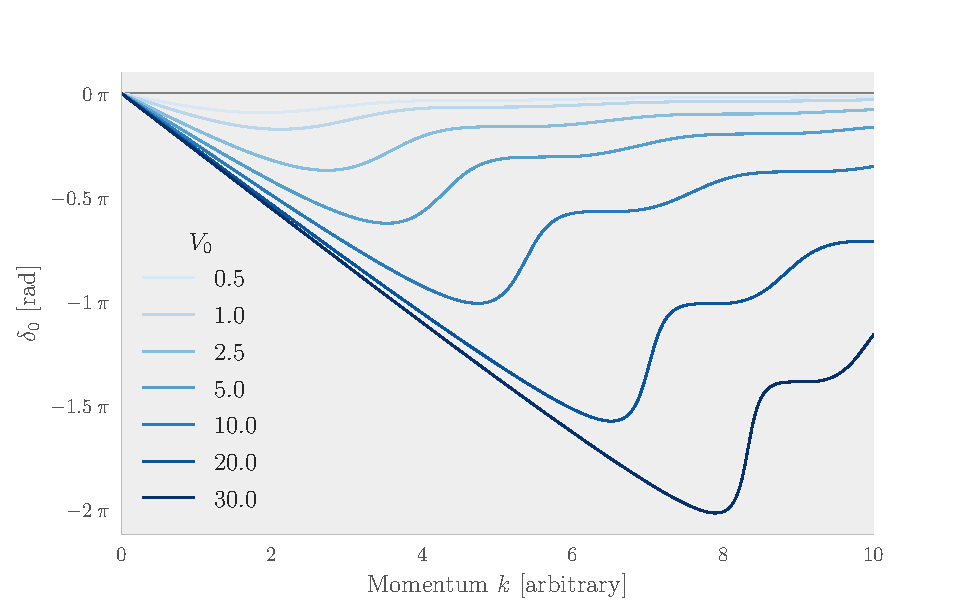
\includegraphics[]{Figures/positive_square_well.pdf}
  \caption{\label{fig:positivesquare}The square well with positive well depths,
    yielding negative phase shifts and no bound states.}
\end{figure}


\subsection{The Reid Potential}

% \begin{figure}[ht]
%   \centering
%   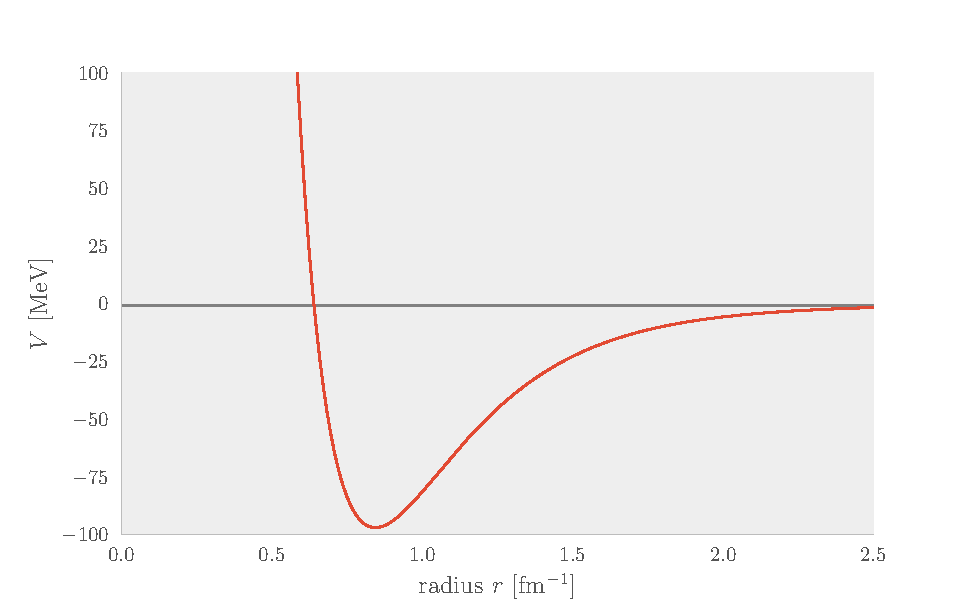
\includegraphics[]{Figures/yukawa.pdf}
%   \caption{\label{fig:yukawa} }
% \end{figure}

\subsubsection{K-Matrix}
The phase shifts for the \(^{1}S_{0}\) partial wave of \(np\)-scattering
obtained through the K-matrix method are shown 
in~\cref{fig:kmatrix}. This is compared to experimental data from the Nijmegen
group, as well as their own pet model \(nijm93\)\cite{PhysRevC.48.792}, also shown in the same figure. There is generally a
good agreement, with all features of the experimental data being replicated; a
rapid rise from 0 to \(\approx 60\degree\), followed by a fall and a sign flip
at \mbox{\(\approx 250\) MeV}. However, the computed phase shift is consistently lower
than the experimental, and lower than \(nijm93\) until the lines cross at
\(300\) MeV.

\begin{figure}[ht!]
  \centering
  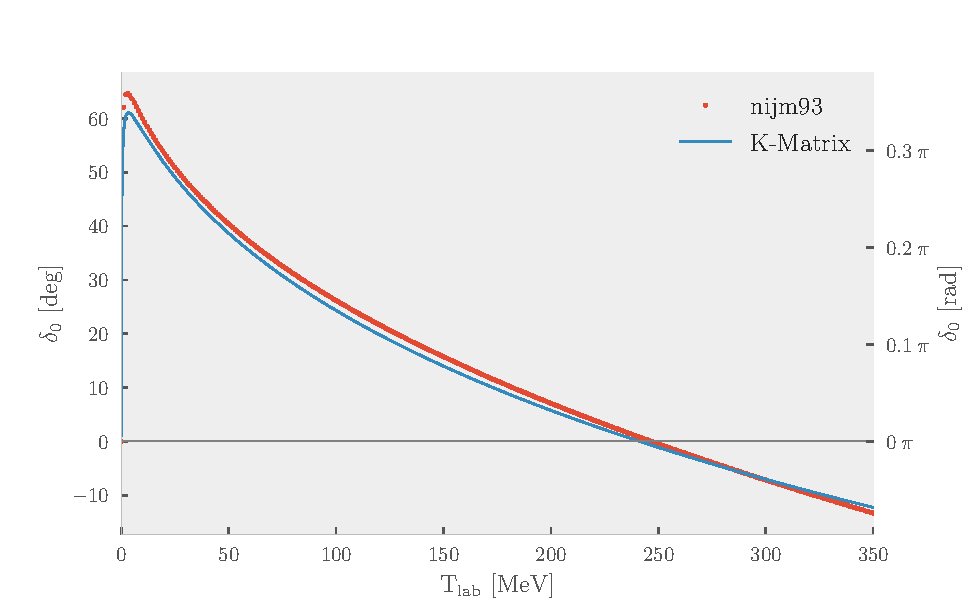
\includegraphics[]{Figures/kmatrix.pdf}
  \caption{\label{fig:kmatrix}Phase shift for \(^{1}S_{0}\) partial wave of
    \(np\)-scattering found by K-matrix calculations using the Reid potential. The experimental data and \(nijm93\) potential fit to
    aforementioned data are also shown, taken from\cite{PhysRevC.48.792}
. There is good agreement, but the
  calculated phase shift is consistently lower than the experimental
  values. 30 mesh points were used in the calculation for each phase shift point.}
\end{figure}

The accuracy of the K-matrix calculations depends on the number of mesh points
used. To determine its influence, different mesh sizes were used to compute the
phase shift at the same energies at the experimental data, and compared to them.
The comparison was made by taking the total mean square error (MSE).
See~\cref{fig:kmatrix_accuracy}. 

Unsurprisingly, the MSE starts off jumping before quickly falling off to a
minimum at about \(25\) mesh points.  As the MSE converges with just a few mesh points, the
discrepancy observed in~\cref{fig:kmatrix} can not be attributed to the method
itself. Increasing the number further gives
negligible improvements. There is, however, an increasing cost in computational
resources.


\begin{figure}[ht!]
  \centering
  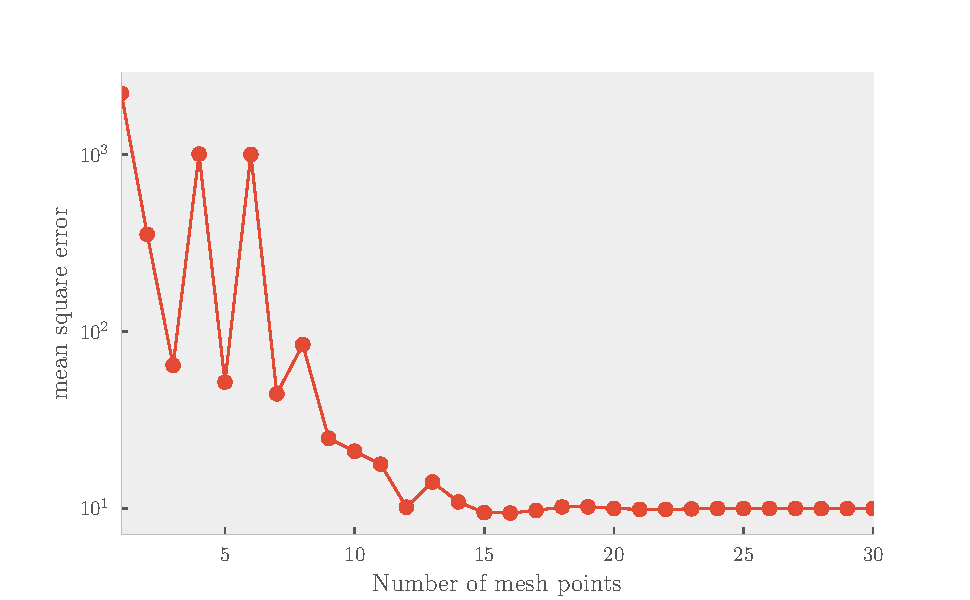
\includegraphics[]{Figures/kmatrix_accuracy}
  \caption{\label{fig:kmatrix_accuracy}The mean square error of the K-Matrix method as a
  function of number of mesh points. The computed values were compared to the
  mean of the experimental values. The For \(n>20\), the error remains near
  constant.}
\end{figure}

The total computation time and amount of allocated bytes used by the K-matrix
method is shown in~\cref{fig:kmatrix_measurements}. As discussed
in~\cref{sec:discret}, both the time and the memory is expected to increase by roughly
\(\mathcal{O}(N^{2})\), \(N\) being the mesh size. Fitting second degree polynomials, we see that this is
indeed roughly the case, with the required time being slightly chaotic due to
the stochastic nature. The
time was measured by repeating each calculation ten times and taking the median.

There is therefore a trade off between the resources required for a calculation
and the accuracy obtained, a trade off that quickly gets increasingly poor,
as no further benefit is obtained after \(\approx 25\) mesh points.

\begin{figure}[ht!]
  \centering
  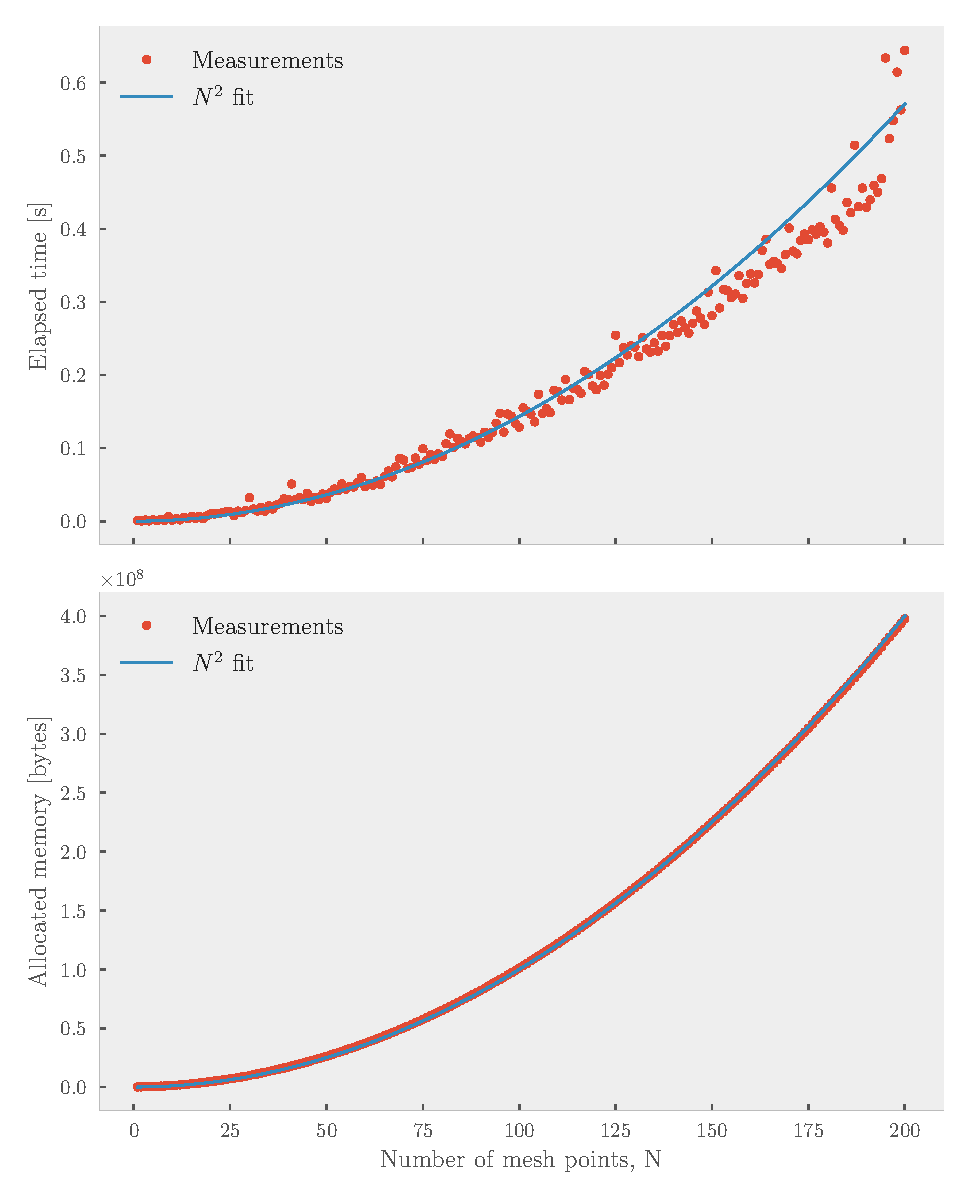
\includegraphics[]{Figures/kmatrix_measurements.pdf}
  \caption{\label{fig:kmatrix_measurements}Resource usage of the K-matrix
    method as a function of number of mesh points. The time shows the median of
    \(10\) repetitions.}
\end{figure}



\subsubsection{VPA}

The second method for obtaining the phase shift from the Reid potential is the
variable phase approach. As before, the results are compared with the Nijmegen results
in~\cref{fig:vpa}, and not unexpectedly, it gives very similar results
as~\cref{fig:kmatrix}.

\begin{figure}[ht!]
  \centering
  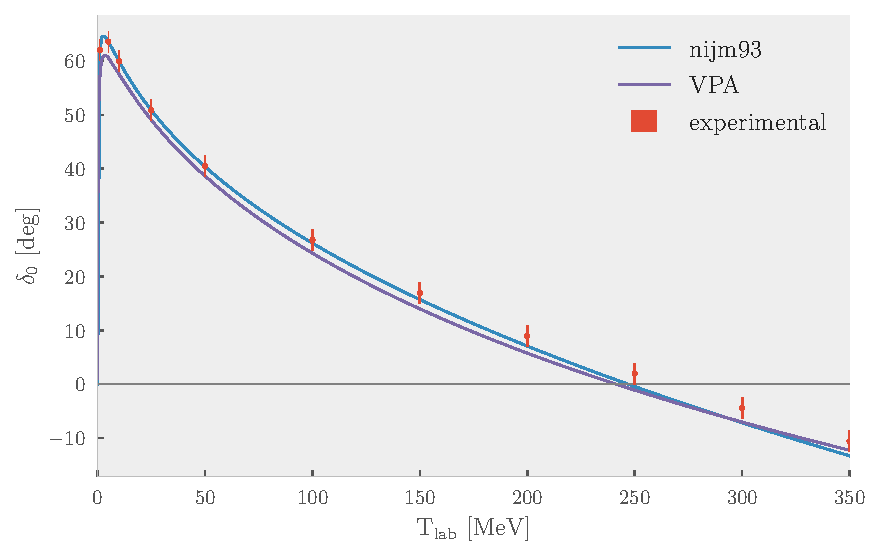
\includegraphics[]{Figures/vpa.pdf}
  \caption{\label{fig:vpa}The resulting \(s\)-wave phase shift from the variable
    phase approach alongside experimental Nijmegen data.}
\end{figure}

VPA requires the cut-off\footnote{I chose the notation \(r_{\text{end}}\) instead of
  the earlier used $\rho$ to underline that $\rho$ is a dummy variable for
  theoretical use, while $r_{\text{end}}$ is a deliberate choice for when to
  stop the integration of the differential equation.} \(r_{\text{end}}\) of the potential to be sufficiently close to infinity
to make the error negligible. Cutting off at low \(r_{\text{end}}\) can be computationally
beneficial, so there is one more a trade off between accuracy and resource
usage. The resulting phase shifts from different cut-off points are shown
in~\cref{fig:rend}. When the cut-off is too small, the potential is effectively
a repulsive potential, yielding a negative phase shift. The phase shift gets
increasingly negative as the interaction ``sees'' more of the repulsive region,
but once the attractive region is included, the phase shift quickly increases
and converges to the far-away solution (\(r_{\text{end}}=15\)).


\begin{figure}[ht!]
  \centering
  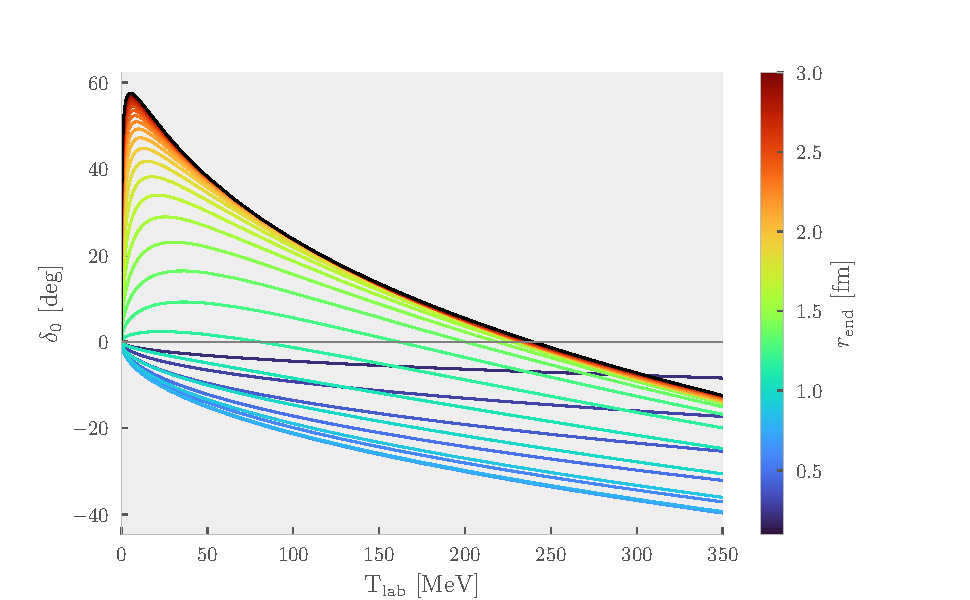
\includegraphics[]{Figures/rend.pdf}
  \caption{\label{fig:rend}The effect of using different cut off points
    \(r_{\mathrm{end}}\) of the potential. Note how the different cut off points
    correspond to the different radii of~\cref{fig:reid}.}
\end{figure}

The resource usage of VPA is significantly more difficult to measure, as the
differential equation is solved by the external package
\textrm{DifferentialEq.jl}, allowing for a range of different parameters and
methods. For completeness' sake, the MSE, time and memory usage as a function of
the step size are shown in the appendix~\cref{fig:vpa_measurements}. The
interesting information is that the time is nearly constant at \(\approx 0.2\)
seconds for the same number of phase shift points as the K-matrix method solved
in~\cref{fig:kmatrix_measurements}. The K-matrix method is therefore
significantly faster, with no loss in accuracy.


\subsubsection{Comparison and Exploration}

The phase shift from both K-matrix calculations and VPA are plotted together
in~\cref{fig:vpa_matrix_compare} alongside the Nijmegen experimental data and
their potential. The nijm93 potential was interpolated with linear interpolation to match up to the
experimental data. The pointwise
relative error is shown in the lower panel. Both curves obtained from the
K-matrix method and VPA are perfectly overlapping, illustrating that they yield
equivalent results of computing the phase shift. Since we already know that VPA
is in agreement with the analytical solutions of the square well, we have
confidence that the K-matrix method too is correctly implemented.


\begin{figure}[ht!]
  \centering
  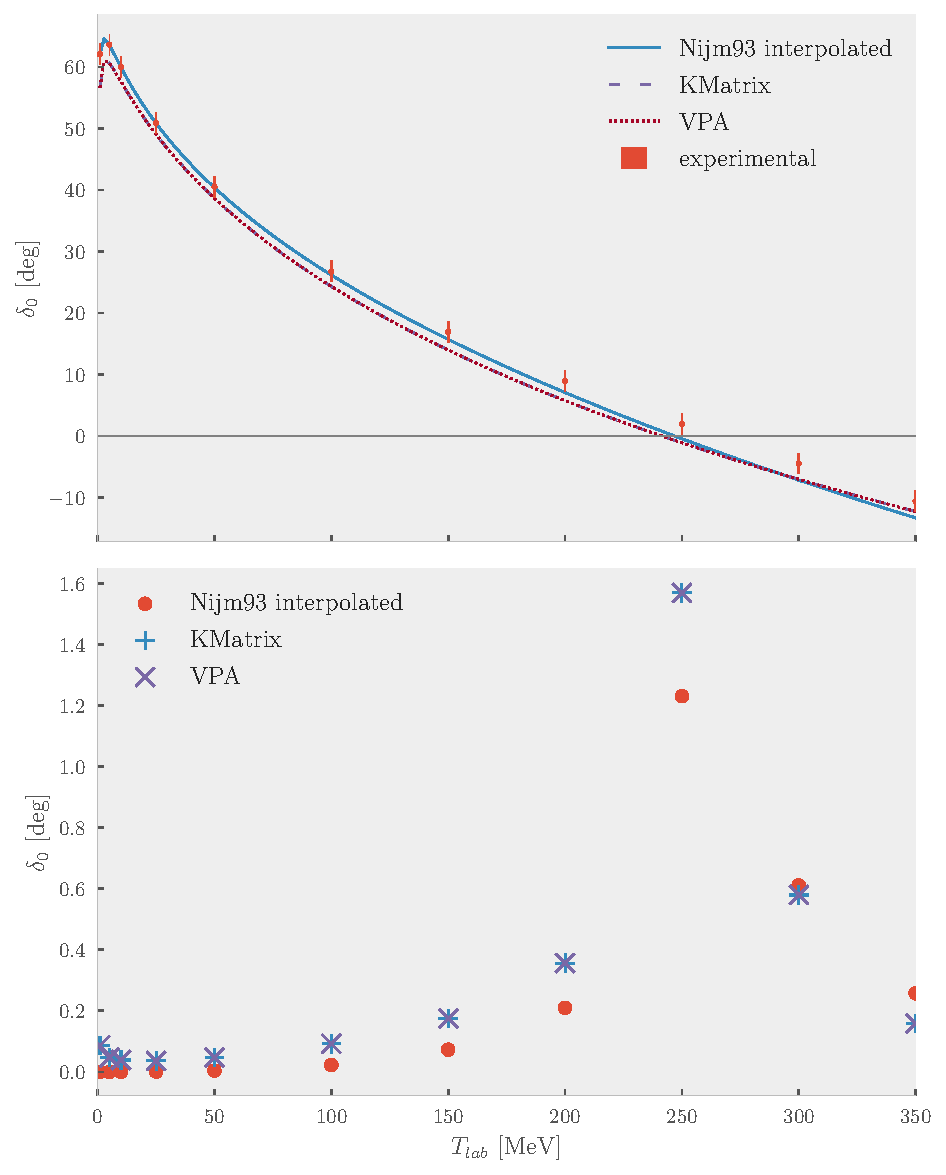
\includegraphics[]{Figures/vpa_kmatrix_compare.pdf}
  \caption{\label{fig:vpa_matrix_compare}The results of K-matrix and VPA using
    good parameters (mesh size of 30, \(r_{\text{end}}\) of 15, default
    diffeq-solver parameters), compared to the \(nijm93\) data. The relative error is
    shown in the lower panel. Only \mbox{\(1 < T_{\mathrm{lab}} < 100\)} MeV are
    included; an arbitrary choice to exclude the jump at \(\approx 0.1 \) MeV
    and the crossing near \(250\) MeV.}
\end{figure}

As the
discrepancy between the theoretical computations and the experimental data can
be attributed to neither the parameters of the methods nor the methods
themselves, the culprit must be the model. The Reid potential was fitted to
\(np\)-scattering data from the \(60\)s and earlier. The later work of the
Nijmegen group, as described in~\cite{PhysRevC.48.792}, used more data obtained
through more accurate methods.

There are, however, some questions arising when examining the Nijmegen
results. Their data was collected from a wide variety of sources, several of
them through private communications. Although they have described their analysis
in detail, some details are rather lacking, one of them being exactly whence the
points shown in~\cref{fig:vpa_matrix_compare} originate. They do not seem to be
experimental data per say, but rather a ``representative sample'' calculated
from the experimental data. Their own \(nijm93\) potential match these points
well at lower energies, getting progressively worse as the energy increases. For
\(T_{\text{lab}}>275\) MeV, the Reid potential yields better results. It is not at
all clear whether the ``experimental'' data points should be held as the golden
yardstick which the potentials ought to be compared. 


% \begin{figure}[ht!]
%   \centering
%   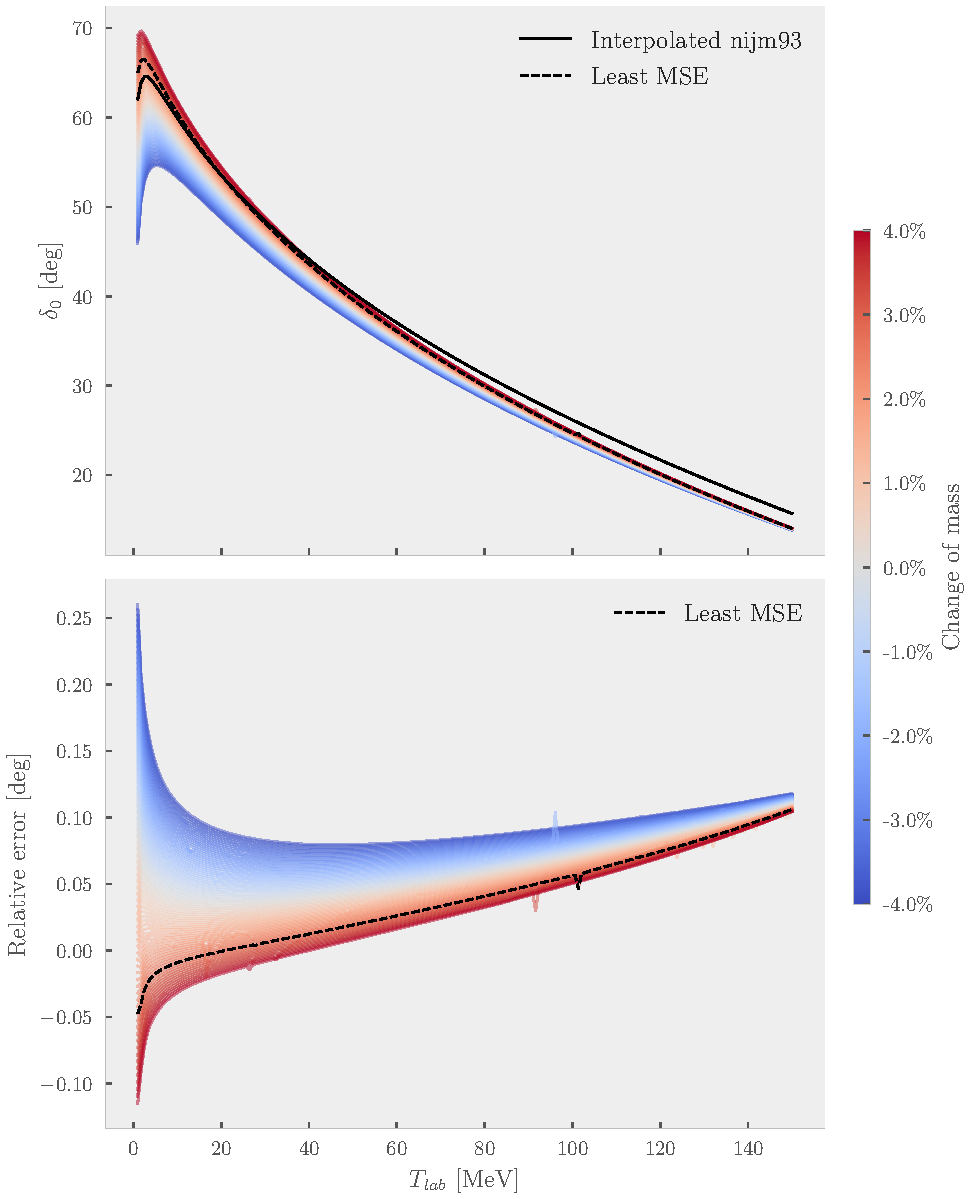
\includegraphics[]{Figures/change_in_mass.pdf}
%   \caption{\label{fig:change_in_mass} A linear parameter search using slightly
%     different masses ranging from \(96\)\% to \(104\)\% of the original mass.
%     The models are compared to \(nijm93\) in the top panel, while the relative
%     error to an interpolated version of \(nijm93\) is shown in the bottom panel.
%     The model with the mass that gives the minimal MSE is shown as dashed line.
%     See the appendix~\cref{fig:optimal_mse} for the MSE curve.}
% \end{figure}

The phase shift curve of the Reid potential has a striking resemblance to the
dashed curves of~\cref{fig:squarewellwave}. From our earlier discussion, it is
easy to suspect
there to be a bound state if the potential was just slightly more
attractive. To examine this, the second term of the Reid potential was increased
by a few percent, yielding the phase shift curves of~\cref{fig:changeV2}. At
\(+3.37\%\) its strength, the phase shift at \(k=0\) jumps up to \(180\degree\),
allowing for a bound state by Levinson's theorem. This is a known experimental
fact, the \(T=0\) singlet not having any bound state in contrast to the bound state of
the \(T=1\) triplet, deuterium. It is striking, however, just how close the
singlet is to obtaining a bound state. 

\begin{figure}[ht!]
  \centering
  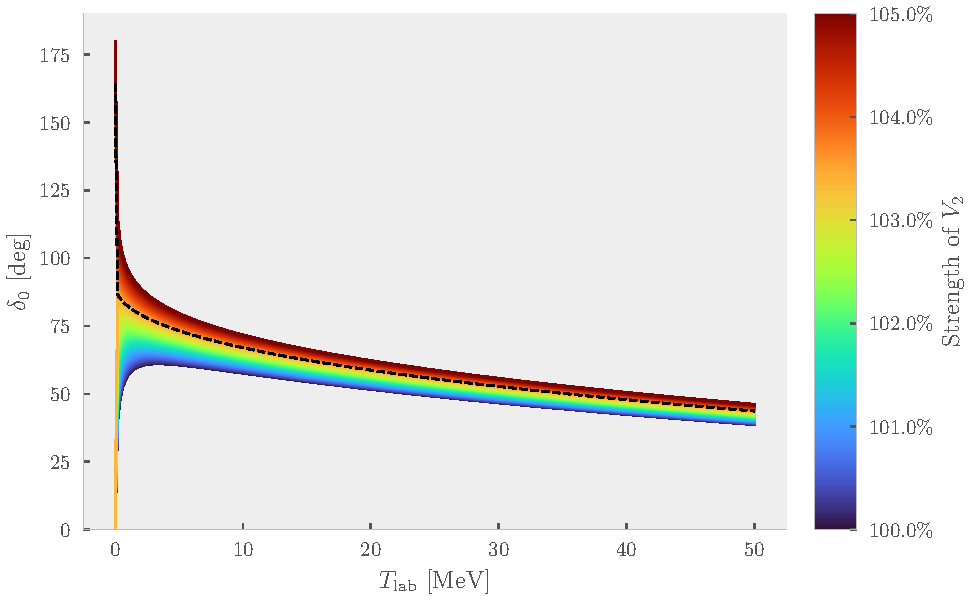
\includegraphics[]{Figures/change_in_V2.pdf}
  \caption{\label{fig:changeV2}The phase shift curves resulting from making the
  Reid potential more attractive by increasing the strength of its second term
  (\(V_{2}=-1650.6\) MeV). The initial blue \(100\%\) denotes its original
  value. At a \(3.37\%\) increase, the curves no longer begin at \(0\degree\),
  but jump to \(180\degree\). This is marked by a dashed line. The apparent lower start point is due to numerical
inaccuracy.}
\end{figure}



%%% Local Variables:
%%% mode: latex
%%% TeX-master: "../main"
%%% TeX-engine: xetex
%%% End:
